\documentclass{beamer}
\usepackage{xeCJK}
\usepackage{listings}
\usepackage{graphicx}
\usepackage{indentfirst}

\title{数据结构第四讲}
\subtitle{树链剖分专题}
\author{丁尧尧}
\institute{上海交通大学}
\date{\today}
\usetheme{PaloAlto}
\setlength{\parindent}{1em}

\begin{document}
	\maketitle
	\begin{frame}{目录}
		\tableofcontents
	\end{frame}
	\section{树链剖分}
		\begin{frame}{解决的问题}
			还记得我们第二讲中提到的那个问题吗?
			\begin{itemize}
				\item 链修改,子树修改,链查询,子树查询
			\end{itemize}
			我们先来解决链修改,链查询的问题。
		\end{frame}
		\begin{frame}{先引入一些概念}
			\begin{definition}
				在一棵有根树上,我们称一个节点$u$的子节点$v$为节点$u$的\textbf{重儿子}当且仅当$v$是所有子节点中大小最大的(如果有多个,则随便选定一个),其余节点称为\textbf{轻儿子}。如果我们对于所有内部节点(有儿子的节点)都选择一个节点作为其重儿子,那么我们就得到了一个轻重链划分,我们称连接节点及其重儿子的边为\textbf{重边},反之则为\textbf{轻边},一条由重边组成的链称为\textbf{重链}。
			\end{definition}
		\end{frame}
		\begin{frame}{重要性质}
			在一个划分下,有如下的性质:
			\begin{theorem}
				树的任意一条路径都可以表示成$O(log(n))$条重链和轻边组成。
			\end{theorem}
			\begin{proof}
				我们只需要证明任意一个节点到根节点的路径最多需要$O(log(n))$条轻边即可。我们考虑从某个节点向上走,每走过一条轻边到达一个点,该点所代表的子树大小至少翻倍,所以要走到根节点,至多经过$O(log(n))$条轻边。
			\end{proof}
		\end{frame}
		\begin{frame}
			我们可以通过调整DFS时子节点的访问顺序,让它先走重儿子,这样任何一条重链就是连续的一段了。那么我们任意一条链(单点算作长度为$1$的重链)都可以由至多$log(n)$条重链表示,从而只需要$log(n)$个区间。(所以树链剖分弄出来的那个序就是一个特殊的DFS序)。
			
			
			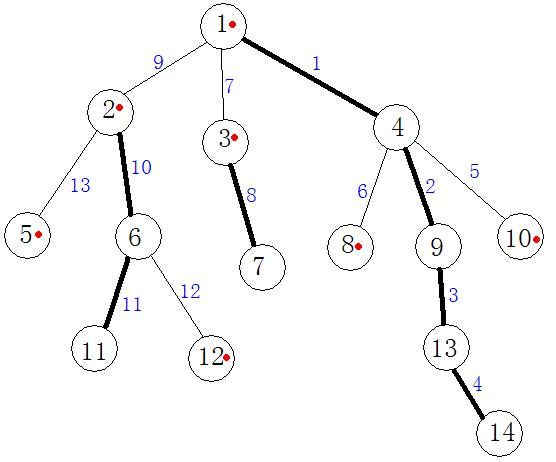
\includegraphics[height=4cm]{tdcp.jpeg}\footnote{摘自starszys的博客}
		\end{frame}
		\begin{frame}
			让我们来看看要把这样一个结构搞出来需要维护些什么东西:
			
			\begin{itemize}
				\item \texttt{siz[u]} 节点$u$的大小
				\item \texttt{dep[u]} 节点$u$到根节点的路径上的点数
				\item \texttt{fat[u]} 节点$u$的父亲
				\item \texttt{son[u]} 节点$u$的重儿子
				\item \texttt{top[u]} 节点$u$只走重边,能走到的深度最小的点
				\item \texttt{in[u]} 节点$u$ 在DFS序中代表的位置,并且也是$u$代表的子树开始的位置
				\item \texttt{out[u]} 节点$u$代表的子树结束的位置
			\end{itemize}
			
			一般而言,前四个可以一次DFS搞定,后三个在第二次DFS时去得到。
		\end{frame}
		\begin{frame}[fragile=singleslide]
			前四个量:
			\begin{verbatim}
void dfs1( int u ) {
    siz[u] = 1;
    for( int t = head[u]; t; t = last[t] ) {
        int v = dest[t];
        if( v == fat[u] ) continue;
        fat[v] = u;
        dep[v] = dep[u]+1;
        dfs(v);
        siz[u] += siz[v];
        if( siz[v] > siz[son[u]] ) son[u] = v;
    }
}
dep[1] = 1;
fat[1] = 1;
dfs1(1);
			\end{verbatim}
		\end{frame}
		\begin{frame}[fragile=singleslide]
			后三个量:
			\begin{verbatim}
void dfs2( int u, int tp ) {
    in[u] = ++idc;
    top[u] = tp;
    if( son[u] ) dfs2( son[u], tp );
    for( int t = head[u]; t; t = last[t] ) {
        int v = dest[t];
        if( v == fat[u] || v == son[u] ) continue;
        dfs2( v, v );
    }
}	
idc = 0;
dfs2(1,1);
			\end{verbatim}
		\end{frame}
		\begin{frame}[fragile=singleslide]
			建出来怎么用呢,一般来说,边权的问题都会先转化成点权的问题。所以下文所有问题都是基于点权的。
			
			链剖最裸的应用是求lca,下面给出代码:
			
			\begin{verbatim}
int lca( int u, int v ) {
    while( top[u] != top[v] ) {
    if( dep[top[u]] < dep[top[v]] ) swap(u,v);
    u = fat[top[u]];
    }
    return dep[u] < dep[v] ? u : v;
}
			\end{verbatim}
			
			这个算法的复杂度是$O(log(n))$的,实际上来看这个应该比倍增求lca常数要小些。
		\end{frame}
		\begin{frame}[fragile=singleslide]
			我们再来看看一个如果涉及线段树时是怎样的:
			\begin{verbatim}
operate_path( int u, int v ) {
    while( top[u] != top[v] ) {
        if( dep[top[u]] < dep[top[v]] ) swap(u,v);
        operate_seg( in[top[u]], in[u] );
        u = fat[top[u]];
    }
    if( dep[u] < dep[v] ) swap( u, v );
    operate_seg( in[v], in[u] );
}
			\end{verbatim}
			
			其中\texttt{operate\_path}表示对路径的一种操作,可以是修改或查询,\texttt{operate\_seg}则是关于线段树的某个操作。
		\end{frame}
		\begin{frame}
			通过上面的学习,我们应该可以解决链修改和链查询的问题了,至于子树修改和子树查询,因为我们得到的序本来就是一种特殊的DFS序,所以可以直接用$[in[u],out[u]]$去操作一个子树的信息。
			
			至此,树形结构的最后一种形式的问题得到解决。但我们解决的仅仅局限于求最值,求和这类很容易维护的信息,像求第K大,求众数,求某个数出现的次数这些问题我们还未解决。求不带修改的子树的第K大我们已经会了,求链上的第K大可以在树上建可持久化线段树解决,求众数可以用莫对(链直接树上莫队,子树转化成求序列上的区间众数直接用莫队),求莫个数出现次数最简单暴力的做法是在每个线段树节点中再维护一个集合。
		\end{frame}
\end{document} 

